\section{Performance}
\label{performance}

In this section, we discuss the real-world performance obtained by running the SIFT detection algorithm as described in section~\ref{sift} and the neural network as described in section~\ref{neural_network}. We chose a relatively old, mid-range laptop to run the tests on as it was the machine that we intended to use for our demo during the poster session. The laptop was a 2012 Macbook equipped with a <CPU>, <RAM>, <GFX>, running on <MAC OS darwin???>.

\subsection{SIFT}
\label{perf_SIFT}

\begin{table}[t]
\caption{SIFT Ratios Matches}
\label{sift_ratios}
\begin{center}
\begin{tabular}{ll}
\multicolumn{1}{c}{\bf RATIO}  &\multicolumn{1}{c}{\bf INCORRECT MATCHES}
\\ \hline \\
0.50             &111 of 196 \\
0.60             &105 of 196 \\
0.70             &100 of 196 \\
0.72             &95 of 196 \\
0.74             &95 of 196 \\
0.76             &91 of 196 \\
0.78             &94 of 196 \\
0.80             &98 of 196 \\
0.90             &102 of 196 \\
\end{tabular}
\end{center}
\end{table}

The SIFT gesture detector was able to run in real-time, although it only had an accuracy of 53.57\%. This relatively low accuracy rate is due to using a training set that is unfavorable towards it. The images used were not cropped to contain only the model hand, and occasionally included a noisy background in the form of the subject's shirt. This proved to be problematic as there were occasionally more keypoints generated for the subject's shirt than their hand (Figure~\ref{kp_noise}) and the matching algorithm would consequently find the best match for the shirt than the hand. This contributed towards the low validation accuracy as the validation set shared the same subjects and consequently the same shirts.

\begin{figure}[h]
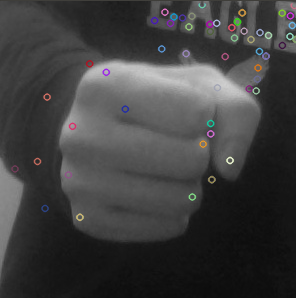
\includegraphics[scale=0.35]{kp_noise.png}
\centering
\caption{Generated keypoints from one training example. There were more keypoints identified for the text on the clothing than the hand.}
\label{kp_noise}
\end{figure}

We considered altering the dataset to better suit SIFT, but ultimately decided against it as we felt that it would produce a similar adverse effect on the neural network and lacked the time to do so. However, we did attempt to run SIFT using HSV color space, but as mentioned in section \ref{sift}, performance dropped to 2 frames per second as opposed to the original 30. As expected, there were more keypoints generated in hue space than in grayscale on the hands due to preserving the orthogonality of the 3 color basis vectors.

\subsection{Neural Network}
\label{perf_NN}
Out of all the networks, network7 performed the best with 100\% training accuracy and 90\% test accuracy.

\begin{figure}[h]
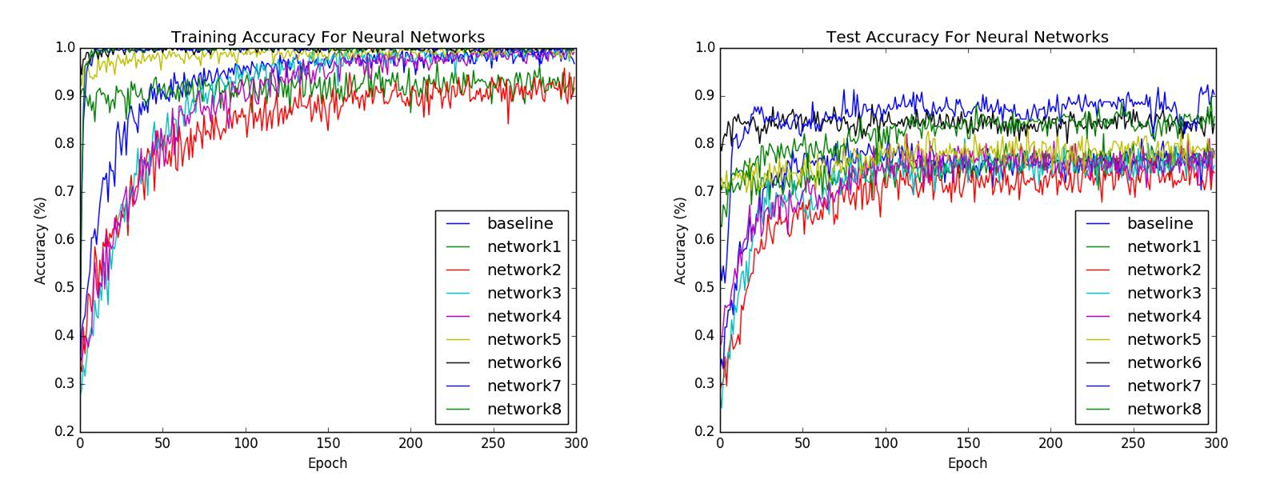
\includegraphics[scale=0.35]{accuracy.png}
\centering
\caption{Training and test accuracy of all the neural networks}
\end{figure}